\documentclass[tikz]{standalone}
\usepackage{tikz-3dplot}

\begin{document}
\tdplotsetmaincoords{60}{120} % Set the main coordinate system angles

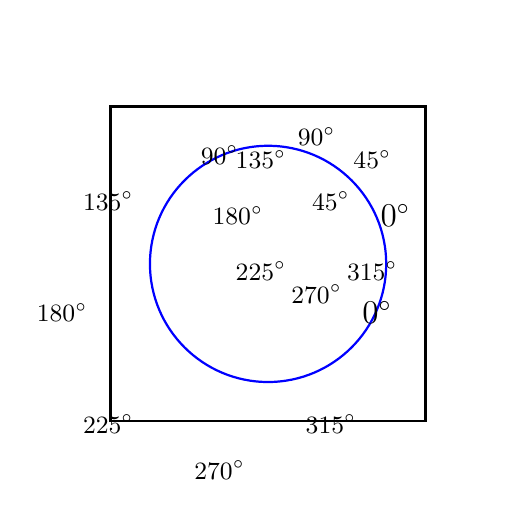
\begin{tikzpicture}[scale=2]
    % Draw the background (white rectangle)
    \fill[white] (-1.5,-1.5) rectangle (1.5,1.5);

    % Draw the cylinder
    \draw[thick, black] (-1,-1) -- (-1,1) -- (1,1) -- (1,-1) -- cycle;
    \draw[thick, black] (-1,-1) -- (1,-1);
    \draw[thick, black] (-1,1) -- (1,1);

    % Draw the sphere
    \draw[thick, blue] (0,0,0) circle[radius=0.75];

    % Draw the arcs and labels around the sphere and cylinder
    \foreach \angle in {0,45,...,315} {
        \pgfmathsetmacro{\x}{cos(\angle)}
        \pgfmathsetmacro{\y}{sin(\angle)}
        \pgfmathsetmacro{\label}{\angle}
        \ifnum\angle=0
            \node at (\x,\y,0.8) {\large $\label^\circ$};
        \else
            \node at (\x,\y,0.8) {\small $\label^\circ$};
        \fi
    }

    % Draw the arcs and labels around the cylinder
    \foreach \angle in {0,45,...,315} {
        \pgfmathsetmacro{\x}{cos(\angle)/2}
        \pgfmathsetmacro{\y}{sin(\angle)/2}
        \pgfmathsetmacro{\label}{\angle}
        \ifnum\angle=0
            \node at (\x,\y,-0.8) {\large $\label^\circ$};
        \else
            \node at (\x,\y,-0.8) {\small $\label^\circ$};
        \fi
    }
\end{tikzpicture}
\end{document}